\documentclass[aps,pra,reprint,groupedaddress,twocolumn,superscriptaddress,linenumbers]{revtex4-2}

\usepackage{graphicx}% Include figure files
\usepackage{dcolumn}% Align table columns on decimal point
\usepackage{bm}% bold math
\usepackage{amsmath}
\usepackage{siunitx}
\usepackage{enumitem}

\begin{document}

\preprint{APS/123-QED}

\title{Atmospheric Metrology for Quantum Networks}
%% the title gives reader a feeling that the article provides a general framework for quantum network, but here we are only using a specific wavelength - we could add a table to introduce different optical clock transition of different ions and list the predicted refractive index offset and compensation performance.

\author{Wei Wu}
\affiliation{Albert-Ludwigs-Universität Freiburg, Physikalisches Institut, Hermann-Herder-Straße 3, 79104 Freiburg, Germany}
\affiliation{EUCOR Centre for Quantum Science and Quantum Computing, University of Freiburg, Hermann-Herder-Straße 3, 79104 Freiburg, Germany}
\author{Tobias Schätz}
\affiliation{Albert-Ludwigs-Universität Freiburg, Physikalisches Institut, Hermann-Herder-Straße 3, 79104 Freiburg, Germany}
\affiliation{EUCOR Centre for Quantum Science and Quantum Computing, University of Freiburg, Hermann-Herder-Straße 3, 79104 Freiburg, Germany}
\author{Ulrich Warring}
\affiliation{Albert-Ludwigs-Universität Freiburg, Physikalisches Institut, Hermann-Herder-Straße 3, 79104 Freiburg, Germany}

\date{\today}

\begin{abstract}
Quantum networks utilizing atomic transitions, such as the \SI{1762}{\nano\meter} line of trapped $^{138}\text{Ba}^+$ ions, face a critical challenge in realistic environments where atmospheric phase noise rapidly degrades quantum coherence. Here we establish a wavelength-specific metrological framework demonstrating that environmental compensation is essential for practical quantum networking. Using quantum-referenced interferometry traceable to a single trapped ion, we analyze \num{89106} measurements to determine the refractive index coefficients of air at \SI{1762}{\nano\meter} with part-per-billion precision. This dataset reveals a significant systematic enhancement in humidity sensitivity compared to standard models, which we attribute to molecular absorption features of water vapor based on first-principles analysis and spectral data. Building on this refined refractive index model, we apply an environmental bookkeeping strategy to an independent set of \num{46999} synchronized measurements across 15 days at a single outdoor location. This post-processed approach suppresses phase noise by \SI{60.20}{\percent} in a representative 12 hours dataset and by \SI{80.97}{\percent} across the full dataset. We identify two distinct suppression regimes, one showing a 560 times reduction in correlation time suitable for quantum gate operations, and another providing sustained 5.3 times noise reduction advantageous for quantum memory applications. This proof-of-principle and post-processed demonstration establishes that wavelength-specific environmental compensation is critical for future quantum networks and provides an algorithmic starting point for future real-time implementations and multi-site validation.
%% if we want to sell this paper in a higher level, the real-time compensation is very necessary to check, otherwise it might leave readers a impression of overselling...
\end{abstract}

\pacs{42.50.-p, 42.25.Bs, 07.60.Ly, 03.67.Hk}

\maketitle

\section{Introduction}

Realizing scalable quantum networks represents a critical milestone for secure quantum communication, distributed quantum computing, and enhanced metrological capabilities \cite{kimble2008quantum,wehner2018quantum,azuma2023quantum}. Trapped-ion systems emerge as promising platforms owing to their exceptional coherence properties, with the \SI{1762}{\nano\meter} transition in $^{138}\text{Ba}^+$ ions being particularly advantageous for optical frequency standards \cite{ludlow2015optical}. However, maintaining quantum phase coherence under realistic atmospheric conditions remains challenging due to refractive index fluctuations induced by temperature, pressure, and humidity variations.

Existing atmospheric refractivity models, while well-characterized for telecommunications wavelengths \cite{ciddor1996refractive, mathar2007refractive}, provide only extrapolated estimates at quantum-critical wavelengths like \SI{1762}{\nano\meter}. Particularly near water vapor absorption features, standard models may significantly underestimate humidity sensitivity due to unaccounted dispersion effects \cite{ptashnik2012water,kochanov2016hitran,gordon2022hitran2020}. This wavelength-specific uncertainty directly impacts the feasibility of environmental compensation strategies for quantum networking.

Here, we demonstrate that precision metrology enables effective suppression of atmospheric phase noise through physical-model-based compensation. Using quantum-referenced interferometry traceable to a single trapped ion, we establish the definitive refractive index coefficients for air at \SI{1762}{\nano\meter} with part-per-billion precision. Our results reveal a systematic enhancement in humidity sensitivity attributable to Kramers-Kronig dispersion near water vapor resonances.

Applying these experimentally determined coefficients to independent field data, we achieve \SI{80.97}{\percent} phase noise reduction over 15-day datasets and identify distinct suppression regimes optimized for quantum memory and gate operations. This post-processed demonstration provides the essential transfer function between environmental parameters and quantum phase stability, establishing environmental bookkeeping as a viable strategy for robust quantum network operation \cite{predehl2012920}.

The compensation approach presented herein utilizes offline feed-forward subtraction based on linear environmental modeling, with validation limited to a single geographic location. Future work will explore real-time implementation and multi-site generalization.

\begin{figure}
\centering
\includegraphics[width=0.45\textwidth]{figures/fig1_nc.eps}
\caption{
Quantum-traceable metrology architecture for precision refractometry at the \SI{1762}{\nano\meter} barium-ion transition wavelength. 
\textbf{(Blue)} Laboratory-based quantum references: a GPS-disciplined oscillator provides a universal timebase, a single trapped Ba$^+$ ion stabilizes the \SI{1762}{\nano\meter} probe laser, and a Rb reference stabilizes the \SI{780}{\nano\meter} reference laser. 
\textbf{(Red)} Field-deployable sensor node: a dual-wavelength interferometer with co-located environmental sensors ($T$, $H$, $P$) measures refractive index changes under realistic outdoor conditions. 
\textbf{(Yellow)} Central analysis unit: processes the validation dataset to establish precise environmental-phase relationships. 
This integrated system bridges quantum-grade stability and field deployment, enabling the part-per-billion precision ($\delta n \sim 1 \times 10^{-9}$) demonstrated in this work.
}
\label{fig:exp_setup}
\end{figure}

\section{Experimental Setup}
\label{sec:experimental_setup}

We developed a quantum-traceable metrology platform to characterize atmospheric refractive index variations at the \SI{1762}{\nano\meter} transition wavelength of $^{138}\text{Ba}^+$ ions. The system architecture, shown in Fig.~\ref{fig:exp_setup}, integrates quantum frequency references with a field-deployable interferometer to achieve part-per-billion precision under realistic outdoor conditions.

The quantum reference system provides absolute frequency stabilization traceable to atomic standards. A single trapped $^{138}\text{Ba}^+$ ion serves as the primary reference for the \SI{1762}{\nano\meter} probe laser, while a rubidium vapor cell stabilizes the \SI{780}{\nano\meter} reference laser via saturation spectroscopy. A GPS-disciplined oscillator ensures precise timing synchronization across all components.

The sensing core consists of a dual-wavelength Michelson interferometer with a \SI{4.2}{\meter} optical path difference, representative of metropolitan-scale quantum link distances. Co-located environmental sensors measure temperature, relative humidity, and atmospheric pressure with calibrated uncertainties of \SI{0.015(2)}{\celsius}, \SI{0.004(1)}{\percent}, and \SI{0.025(3)}{\hecto\pascal}, respectively. The complete assembly was deployed outdoors to capture natural atmospheric variations spanning \SIrange{15}{35}{\celsius}, \SIrange{20}{45}{\percent} relative humidity, and \SIrange{965}{1000}{\hecto\pascal}.

A centralized data acquisition system records synchronized measurements from all sensors, with each optical fringe measurement timestamped to its corresponding environmental conditions. This integrated design enables direct correlation between atmospheric parameters and refractive index changes, forming the basis for the precision coefficient determination presented in the following sections. Detailed instrument specifications and data processing methodologies are provided in Appendix~\ref{app:experimental}.

\begin{figure}
\centering
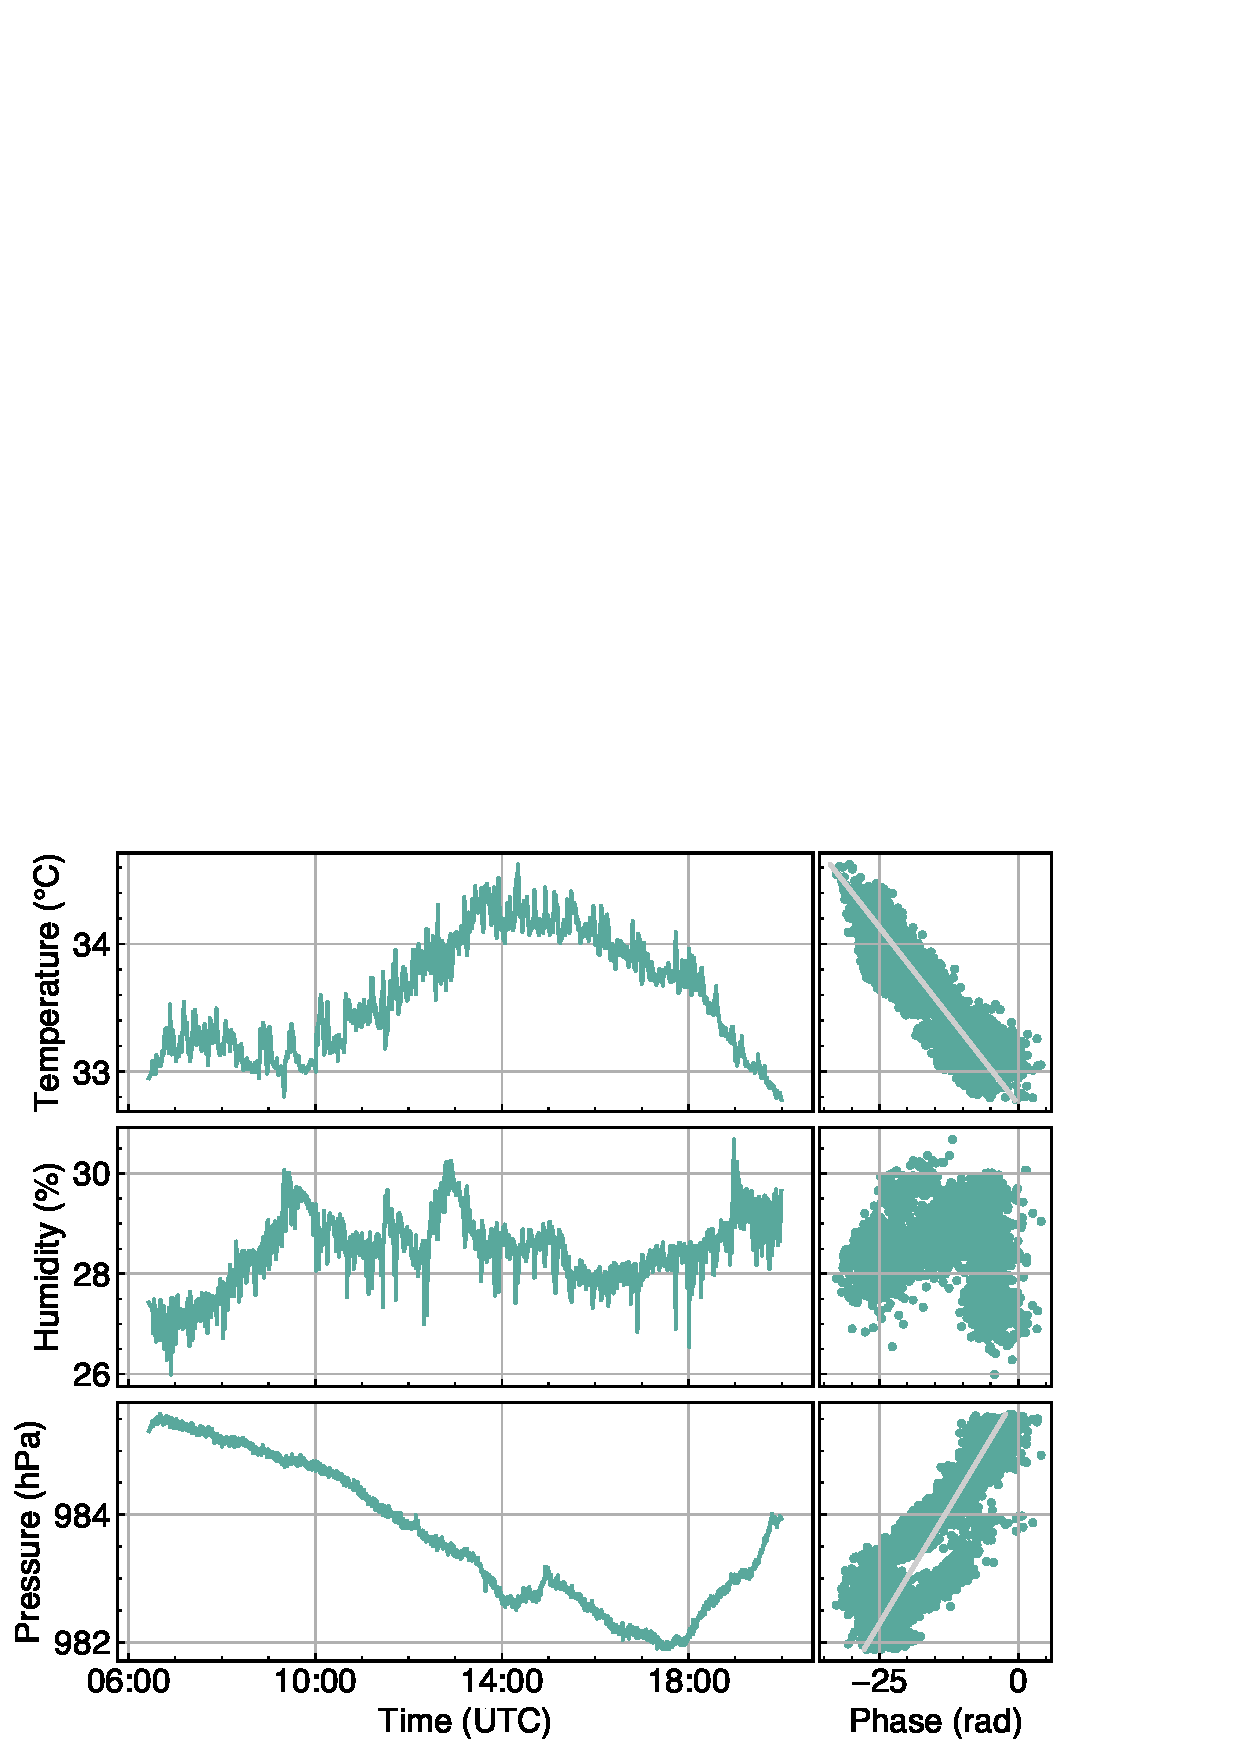
\includegraphics[width=0.48\textwidth]{figures/fig2_new.pdf}
\caption{
Environmental dynamics and their distinct correlations with quantum phase noise.
\textbf{(a--c)} Synchronous \SI{14}{\hour} time-series measurements from the training dataset of atmospheric temperature (\SIrange{33}{34.5}{\celsius}), relative humidity (\SIrange{26}{31}{\percent}), and pressure (\SIrange{982}{986}{\hecto\pascal}) from the training dataset.
\textbf{(d--f)} Quantitative correlation analysis between each environmental parameter and the resulting refractive index change. Phase noise exhibits a strong linear dependence on temperature ($R^{2} = 0.828$) and pressure ($R^{2} = 0.751$). The humidity-phase relationship, however, displays a characteristic non-linear pattern, deviating significantly from simple linear modeling. This systematic deviation, occurring within the measurement uncertainty region, underscores the necessity for the precision humidity coefficient reported herein and reveals a deterministic error source that would scale linearly with quantum link distance.
}
\label{fig:environmental_dynamics}
\end{figure}
%% here we need a table to illuminate the nonlinear fit result of the humdity dependence, otherwise one may get confused, if you realise it is non-linear, why not fit it with non-linear models?

\section{Results}
\label{sec:results}

\subsection{Environmental Dynamics as the Dominant Source of Phase Noise}
\label{sec:environmental_dynamics}

Measurement of the training dataset, comprising \num{89106} synchronized records (representative samples in Tab.~\ref{tab:raw_data_sample}), directly quantifies atmospheric phase noise. Figure~\ref{fig:environmental_dynamics} illustrates a representative \SI{14}{\hour} time series, showing environmental variations that translate to significant phase excursions exceeding \SI{35}{\radian} peak-to-peak. This level of phase instability would severely degrade quantum coherence in outdoor links.

Correlation analysis reveals distinct relationships between each environmental parameter and the resulting refractive index change. While temperature and pressure exhibit strong linear correlations ($R^{2} = 0.828$ and $0.751$, respectively), the humidity-phase relationship displays systematic deviations from linearity within the measurement uncertainty. This nonlinearity, evident in Fig.~\ref{fig:environmental_dynamics}e, signals a complex coupling mechanism that necessitates precise coefficient determination.

\subsection{Precision Determination of Refractive Index Coefficients}
\label{sec:coefficient_determination}

The refractive index at \SI{1762}{\nano\meter} was determined differentially against the well-characterized index at \SI{780}{\nano\meter} using the relation:
\begin{equation}
\label{eq:n1762}
    n_{1762} = \frac{n_{780}}{\text{Ratio}} \frac{f_{780}}{f_{1762}}
\end{equation}
where $n_{780}$ is calculated from environmental parameters via the Ciddor equation and Ratio is the measured fringe count ratio $N_{1762}/N_{780}$.

Multivariate linear regression on the training dataset yielded the coefficients summarized in Tab.~\ref{tab:suppression_coefficients}. The linear model exhibits exceptional goodness-of-fit, with a coefficient of determination of $R^2 = 0.996$ and a highly significant F-statistic of $7.530 \times 10^6$ ($p < 0.001$). The residual standard error is $\sigma_n \approx \SI{1.2e-9}{}$, which is commensurate with the measurement precision and indicates that the linear model captures the dominant relationships between environmental parameters and refractive index.

The temperature and pressure coefficients show excellent agreement ($<\SI{1}{\percent}$ deviation) with established models, validating the measurement precision. However, the humidity coefficient exhibits a significant enhancement compared to model predictions, as detailed in Tab.~\ref{tab:model_comparison}. This discrepancy prompted further investigation into its physical origin.

\subsection{Physical Origin of Humidity Sensitivity Enhancement}
\label{sec:humidity_origin}

Figure~\ref{fig:humidity_discrepancy}a compares the measured humidity sensitivity with predictions from standard atmospheric models, revealing a consistent underprediction. Spectral analysis (Fig.~\ref{fig:humidity_discrepancy}b) identifies the proximity of the \SI{1762}{\nano\meter} wavelength to strong water vapor absorption lines at \SI{1761.0405}{\nano\meter} and \SI{1762.4852}{\nano\meter}.

A first-principles Kramers-Kronig calculation, detailed in Appendix~\ref{app:dispersion}, accounts for dispersion effects near these resonances. The calculation predicts a dispersion contribution of $\Delta n_{\text{disp}} = \SI{-2.35e-9}{\per\percent}$ at \SI{1762}{\nano\meter}, corresponding to a \SI{15.3}{\percent} enhancement over the pure replacement effect. The resulting theoretical humidity sensitivity agrees with our experimental measurement within \SI{0.5}{\percent}, confirming dispersion as the dominant mechanism for the observed enhancement.

\subsection{Multi-Timescale Noise Suppression Performance}
\label{sec:subtraction}

Applying the experimentally determined coefficients to the independent validation dataset demonstrates significant noise suppression across temporal scales relevant to quantum applications as shown in Fig.~\ref{fig:timeseries_comparison}.

For long-term stability over \SI{15}{\day}, representative of quantum memory coherence times, the environmental bookkeeping achieves \SI{80.97}{\percent} phase noise reduction. The phase standard deviation decreases from \SI{17.938}{\radian} to \SI{3.414}{\radian} (a 5.3$\times$ improvement). Consequently, compliance with the $\pi/8$ QEC threshold increases from \SI{1.2}{\percent} to \SI{9.7}{\percent} of the operational time \cite{preskill1998reliable,fowler2012surface, terhal2015quantum}. The autocorrelation time reduces from \SI{5668}{\second} to \SI{302}{\second}, indicating suppressed long-range correlations.

For short-term dynamics over \SI{12}{\hour}, critical for quantum gate operations, the method provides \SI{60.20}{\percent} noise reduction ($\sigma_\phi$: \SI{6.548}{\radian} $\rightarrow$ \SI{2.606}{\radian}, 2.5$\times$). More significantly, the autocorrelation time dramatically shortens from \SI{560}{\second} to \SI{1}{\second}, effectively whitening the noise spectrum. This transformation improves the threshold compliance from \SI{3.3}{\percent} to \SI{13.3}{\percent}. The distinct performance regimes highlight the adaptability of the approach to different quantum application requirements.

\begin{table*}
\centering
\caption{Representative sample of synchronized measurement data from the dual-wavelength interferometer. The reference refractive index $n_{780}$ is calculated from the environmental parameters using the Ciddor equation \cite{ciddor1996refractive}. The target refractive index $n_{1762}$ is then derived from the measured fringe count ratio and the known frequency ratio using Eq.~\ref{eq:n1762}.}
\begin{ruledtabular}	
\begin{tabular}{cccccccc}
{Time (UTC)} & {$T$ (\si{\celsius})} & {$H$ (\si{\percent})} & {$P$ (\si{\hecto\pascal})} & {$N_{780}/N_{1762}$} & {$n_{1762}$} & Role & Used in\\
\colrule
... & ... & ... & ... & ... & ... & ... \\
2025-01-01 00:02:54 & 17.69 & 33.49 & 997.039 & 2.258486 & 1.000268 & Training & Sec.~\ref{sec:environmental_dynamics}, \ref{sec:coefficient_determination}; Fig.~\ref{fig:environmental_dynamics}, \ref{fig:humidity_discrepancy}; Tab.~\ref{tab:suppression_coefficients}, \ref{tab:model_comparison} \\
2025-01-01 00:05:37 & 17.70 & 33.68 & 997.194 & 2.258486 & 1.000268 & Training& Sec.~\ref{sec:environmental_dynamics}, \ref{sec:coefficient_determination}; Fig.~\ref{fig:environmental_dynamics}, \ref{fig:humidity_discrepancy}; Tab.~\ref{tab:suppression_coefficients}, \ref{tab:model_comparison} \\
2025-01-01 00:06:26 & 17.70 & 33.53 & 997.194 & 2.258488 & 1.000267 & Training& Sec.~\ref{sec:environmental_dynamics}, \ref{sec:coefficient_determination}; Fig.~\ref{fig:environmental_dynamics}, \ref{fig:humidity_discrepancy}; Tab.~\ref{tab:suppression_coefficients}, \ref{tab:model_comparison} \\
2025-01-01 00:07:04 & 17.70 & 33.75 & 997.305 & 2.258486 & 1.000268 & Training& Sec.~\ref{sec:environmental_dynamics}, \ref{sec:coefficient_determination}; Fig.~\ref{fig:environmental_dynamics}, \ref{fig:humidity_discrepancy}; Tab.~\ref{tab:suppression_coefficients}, \ref{tab:model_comparison} \\
2025-01-01 00:07:30 & 17.70 & 33.67 & 997.325 & 2.258487 & 1.000268 & Training& Sec.~\ref{sec:environmental_dynamics}, \ref{sec:coefficient_determination}; Fig.~\ref{fig:environmental_dynamics}, \ref{fig:humidity_discrepancy}; Tab.~\ref{tab:suppression_coefficients}, \ref{tab:model_comparison} \\
... & ... & ... & ... & ... & ... & ... \\
%2025-01-11 17:21:09 & 19.07 & 32.25 & 996.631 & 2.258487 & 1.000266 & Training & Section~\ref{sec:coefficient_determination} \\
%2025-01-11 17:21:22 & 19.07 & 32.41 & 996.575 & 2.258487 & 1.000266 & Training & Section~\ref{sec:coefficient_determination} \\
%2025-01-11 17:21:36 & 19.08 & 31.97 & 996.620 & 2.258487 & 1.000266 & Training & Section~\ref{sec:coefficient_determination} \\
%2025-01-11 17:21:48 & 19.08 & 32.25 & 996.675 & 2.258487 & 1.000266 & Training & Section~\ref{sec:coefficient_determination} \\
%2025-01-11 17:22:00 & 19.09 & 31.88 & 996.692 & 2.258488 & 1.000266 & Training & Section~\ref{sec:coefficient_determination} \\
2025-06-16 19:41:56 & 29.78 & 28.54 & 994.564 & 2.258488 & 1.000255 & Training & Sec.~\ref{sec:coefficient_determination}; Fig.~\ref{fig:humidity_discrepancy}; Tab.~\ref{tab:suppression_coefficients}, \ref{tab:model_comparison} \\
2025-06-16 19:42:13 & 29.77 & 28.42 & 994.596 & 2.258487 & 1.000256 & Training & Sec.~\ref{sec:coefficient_determination}; Fig.~\ref{fig:humidity_discrepancy}; Tab.~\ref{tab:suppression_coefficients}, \ref{tab:model_comparison} \\
2025-06-16 19:42:26 & 29.79 & 28.49 & 994.657 & 2.258488 & 1.000256 & Training & Sec.~\ref{sec:coefficient_determination}; Fig.~\ref{fig:humidity_discrepancy}; Tab.~\ref{tab:suppression_coefficients}, \ref{tab:model_comparison} \\
2025-06-16 19:42:38 & 29.79 & 28.40 & 994.657 & 2.258488 & 1.000255 & Training & Sec.~\ref{sec:coefficient_determination}; Fig.~\ref{fig:humidity_discrepancy}; Tab.~\ref{tab:suppression_coefficients}, \ref{tab:model_comparison} \\
2025-06-16 19:42:52 & 29.78 & 28.40 & 994.657 & 2.258488 & 1.000256 & Training & Sec.~\ref{sec:coefficient_determination}; Fig.~\ref{fig:humidity_discrepancy}; Tab.~\ref{tab:suppression_coefficients}, \ref{tab:model_comparison} \\
%2025-07-08 18:13:02 & 29.53 & 23.72 & 986.666 & 2.258486 & 1.000254 & Training & Section~\ref{sec:coefficient_determination} \\
%2025-07-08 18:13:27 & 29.57 & 24.00 & 986.654 & 2.258487 & 1.000254 & Training & Section~\ref{sec:coefficient_determination} \\
%2025-07-08 18:13:40 & 29.54 & 24.24 & 986.662 & 2.258488 & 1.000254 & Training & Section~\ref{sec:coefficient_determination} \\
%2025-07-08 18:20:26 & 29.34 & 24.08 & 986.744 & 2.258487 & 1.000254 & Training & Section~\ref{sec:coefficient_determination} \\
%2025-07-08 18:20:50 & 29.33 & 24.38 & 986.671 & 2.258488 & 1.000254 & Training & Section~\ref{sec:coefficient_determination} \\
%... & ... & ... & ... & ... & ... & ... \\
%2025-08-04 22:00:06 & 26.90 & 31.56 & 989.117 & 2.258488 & 1.000257 & Validation & Validation \\
%2025-08-04 22:00:19 & 26.89 & 31.47 & 989.060 & 2.258488 & 1.000256 & Validation & Validation \\
%2025-08-04 22:00:31 & 26.90 & 31.35 & 989.060 & 2.258488 & 1.000257 & Validation & Validation \\
%2025-08-04 22:00:44 & 26.91 & 31.46 & 989.133 & 2.258488 & 1.000256 & Validation & Validation \\
%2025-08-04 22:00:56 & 26.92 & 31.28 & 989.045 & 2.258488 & 1.000257 & Validation & Validation \\
... & ... & ... & ... & ... & ... & ... \\
2025-08-20 20:31:49 & 28.22 & 36.72 & 978.948 & 2.258488 & 1.000252 & Validation & Sec.~\ref{sec:subtraction}; Fig.~\ref{fig:timeseries_comparison} \\
2025-08-20 20:32:40 & 28.30 & 36.66 & 978.987 & 2.258488 & 1.000253 & Validation & Sec.~\ref{sec:subtraction}; Fig.~\ref{fig:timeseries_comparison} \\
2025-08-20 20:33:31 & 28.30 & 36.83 & 978.987 & 2.258486 & 1.000254 & Validation & Sec.~\ref{sec:subtraction}; Fig.~\ref{fig:timeseries_comparison} \\
2025-08-20 20:36:18 & 28.33 & 35.83 & 978.922 & 2.258486 & 1.000253 & Validation & Sec.~\ref{sec:subtraction}; Fig.~\ref{fig:timeseries_comparison} \\
2025-08-20 20:37:37 & 28.23 & 36.50 & 979.016 & 2.258488 & 1.000253 & Validation & Sec.~\ref{sec:subtraction}; Fig.~\ref{fig:timeseries_comparison} \\
... & ... & ... & ... & ... & ... & ... \\
\end{tabular}
\end{ruledtabular}
\label{tab:raw_data_sample}
\end{table*}

\begin{figure}
\centering
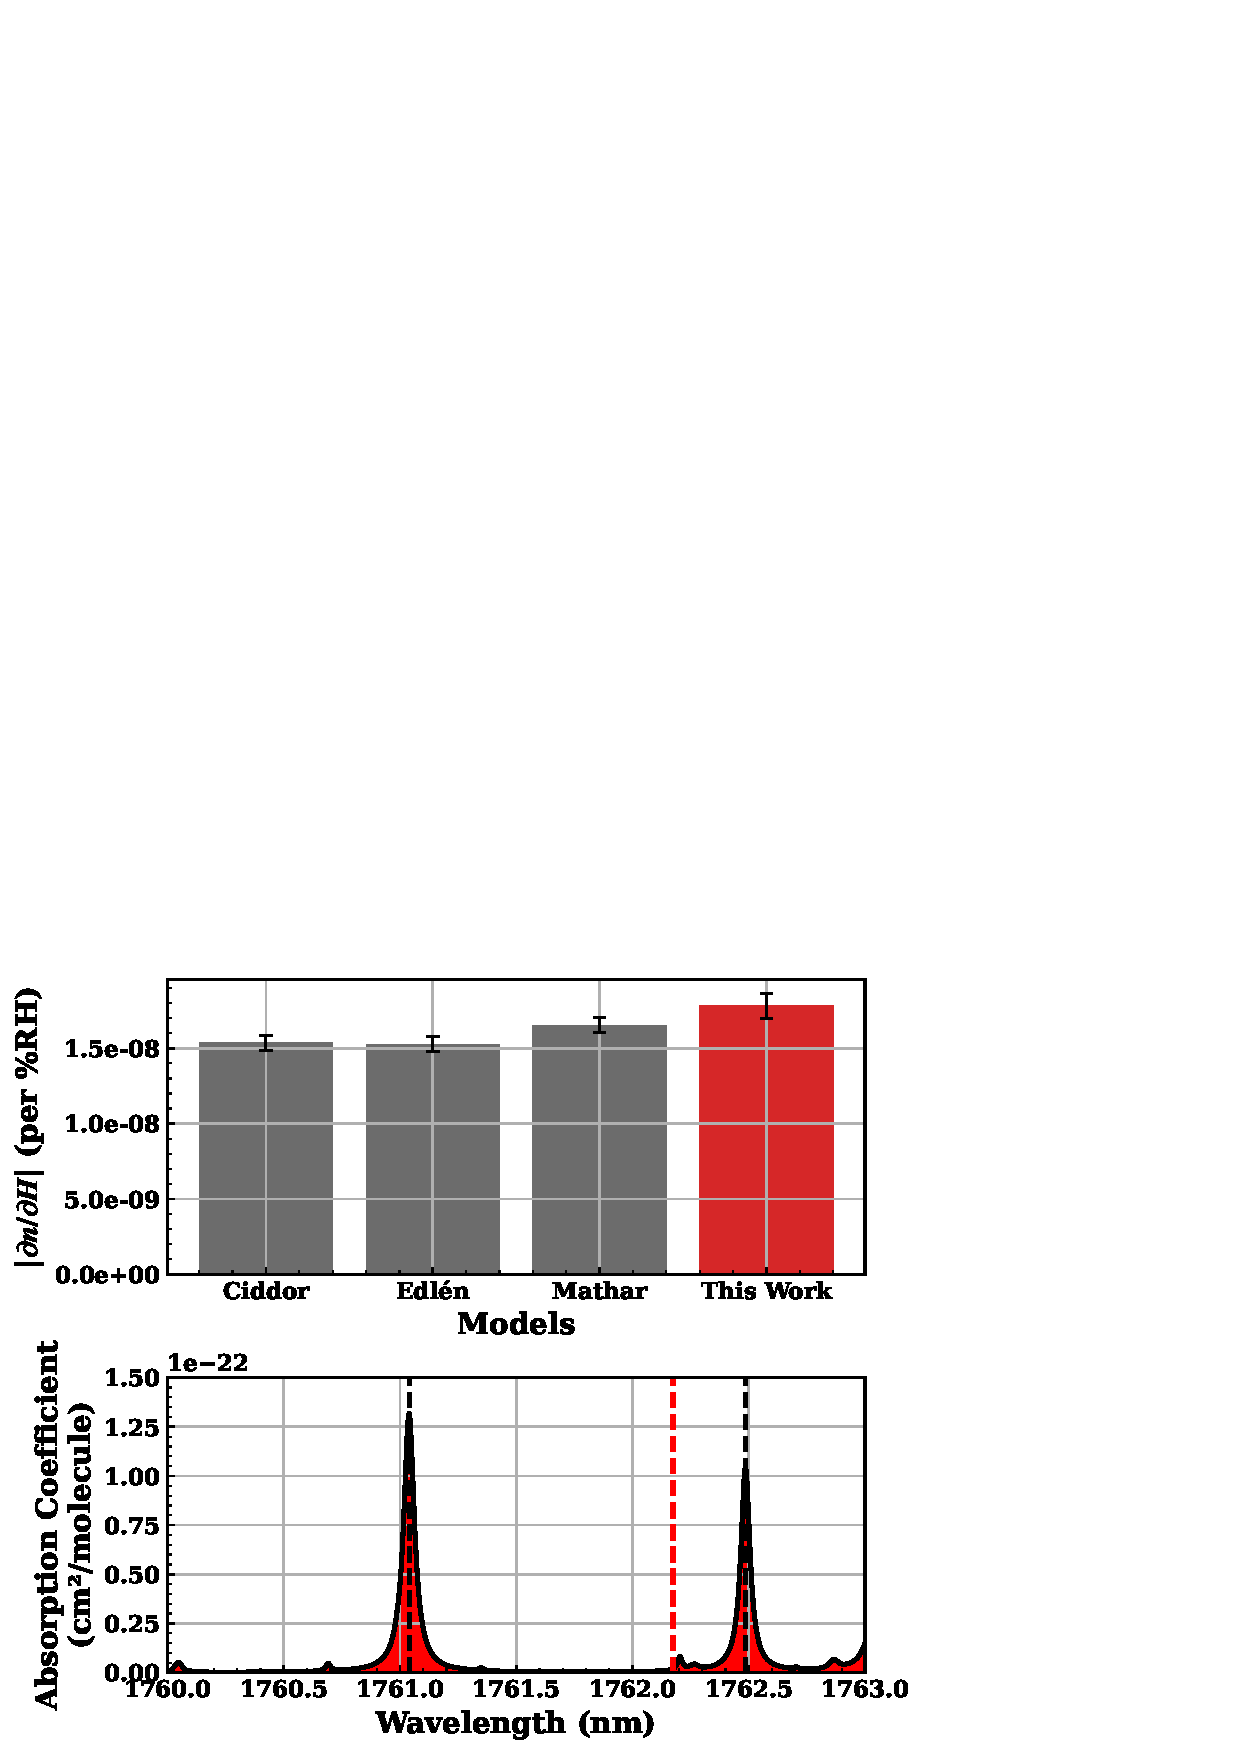
\includegraphics[width=0.45\textwidth]{figures/fig3_humidity_discrepancy.pdf}
\caption{
Systematic discrepancy in humidity sensitivity and its physical origin at \SI{1762}{\nano\meter}.
\textbf{(a)} Comparison of the experimentally derived humidity sensitivity coefficient with predictions from established empirical models. A significant enhancement as shown in Tab.~\ref{tab:model_comparison} is identified, while excellent agreement ($<\SI{1}{\percent}$ deviation) is found for temperature and pressure coefficients.
\textbf{(b)} Spectral analysis showing water vapor absorption features in the vicinity of the quantum-critical wavelength. The \SI{1762}{\nano\meter} transition lies between two strong absorption peaks at \SI{1761.0405}{\nano\meter} and \SI{1762.4852}{\nano\meter}, creating ideal conditions for Kramers-Kronig enhanced dispersion. Our first-principles calculation, performed over the full spectral range from \SI{1}{\micro\meter} to \SI{50}{\micro\meter}, explains the observed \SI{15.3}{\percent} increase in humidity sensitivity compared to the Ciddor model, or other standard atmospheric models detailed in Tab.~\ref{tab:model_comparison}.
}
\label{fig:humidity_discrepancy}
\end{figure}

\begin{table}
\centering
\caption{\label{tab:suppression_coefficients}
Comprehensive Regression Analysis Results for the Refractive Index of Air at \SI{1762}{\nano\meter}. The 95\% confidence intervals (CI) were calculated using HAC standard errors to account for observed temporal dependencies in the residuals.}
\begin{ruledtabular}
\begin{tabular}{lcccc}
Parameter & Coefficient & {95\% CI} \\
\colrule
Temperature ($\alpha_T$) & $-8.940 \times 10^{-7}$ & $[-8.942, -8.938] \times 10^{-7}$ \\
Humidity ($\alpha_H$) & $-1.780 \times 10^{-8}$ & $[-1.796, -1.764] \times 10^{-8}$ \\
Pressure ($\alpha_P$) & $2.569 \times 10^{-7}$ & $[2.557, 2.581] \times 10^{-7}$ \\
\end{tabular}
\end{ruledtabular}
\end{table}

% in case we need more complete model...
% \begin{table}
% \centering
% \caption{\label{tab:suppression_coefficients}
% Refractive Index Coefficients for Air at \SI{1762}{\nano\meter} from Optimal Nonlinear Model.}
% \begin{ruledtabular}
% \begin{tabular}{lcccc}
% Parameter & Coefficient & {95\% CI} & Significance \\
% \colrule
% Temperature ($\alpha_T$) & $-8.940 \times 10^{-7}$ & $[-8.942, -8.938] \times 10^{-7}$ & $p < 0.001$ \\
% Humidity ($\alpha_H$) & $-1.780 \times 10^{-8}$ & $[-1.796, -1.764] \times 10^{-8}$ & $p < 0.001$ \\
% Pressure ($\alpha_P$) & $2.569 \times 10^{-7}$ & $[2.557, 2.581] \times 10^{-7}$ & $p < 0.001$ \\
% Humidity$^2$ ($\alpha_{H^2}$) & $1.24 \times 10^{-10}$ & $[1.19, 1.29] \times 10^{-10}$ & $p < 0.001$ \\
% $T \times H$ ($\alpha_{T\times H}$) & $3.89 \times 10^{-9}$ & $[3.85, 3.93] \times 10^{-9}$ & $p < 0.001$ \\
% \end{tabular}
% \end{ruledtabular}
% \end{table}


\begin{table}
\centering
\caption{\label{tab:model_comparison}Comparison of humidity sensitivity coefficients. Discrepancies are calculated relative to our experimental measurement.}
\begin{ruledtabular}
\begin{tabular}{lccc}
Model & $\partial n/\partial H$ (\si{\per\percent}) & Discrepancy (\si{\per\percent}) & Relative Error \\
\hline
\textbf{This work} & $\mathbf{-1.780 \times 10^{-8}}$ & -- & -- \\
Ciddor \cite{ciddor1996refractive} & $-1.537 \times 10^{-8}$ & $\SI{-2.43e-9}{}$ & \SI{+15.8}{\percent} \\
Edlén \cite{edlen1966refractive} & $-1.526 \times 10^{-8}$ & $\SI{-2.54e-9}{}$ & \SI{+16.6}{\percent} \\
Mathar \cite{mathar2007refractive} & $-1.653 \times 10^{-8}$ & $\SI{-1.27e-9}{}$ & \SI{+7.7}{\percent} \\
\end{tabular}
\end{ruledtabular}
\end{table}

\begin{figure*}
\centering
\includegraphics[width=0.9\textwidth]{figures/combined_figure.png}
\caption{
Multi-scale phase noise characterization and post-processed (offline) suppression efficacy for quantum applications. 
\textbf{(a)} Long-term (\SI{15}{\day}) phase stability using the full validation dataset: time-domain performance showing environmental noise mitigation, with gray shaded region indicating the fault-tolerant threshold. 
\textbf{(b)} Long-term autocorrelation analysis: correlation time reduced from \SI{5668}{\second} to \SI{302}{\second}. 
\textbf{(c)} Long-term spectral characterization: power spectral density demonstrating substantial low-frequency noise suppression. 
\textbf{(d)} Short-term (\SI{12}{\hour}) phase dynamics from the validation dataset: optimized performance for quantum gate operations, with gray shaded region indicating the fault-tolerant threshold. 
\textbf{(e)} Short-term autocorrelation: dramatic noise whitening with correlation time reduced from \SI{560}{\second} to \SI{1}{\second}. 
\textbf{(f)} Short-term spectral analysis: frequency-domain transformation revealing noise structure modification. 
Key performance metrics: Long-term noise reduction of \SI{80.97}{\percent} ($\sigma_\phi$: \SI{17.938}{\radian} $\rightarrow$ \SI{3.414}{\radian}, 5.3$\times$) optimized for quantum memory applications. Short-term suppression achieves \SI{60.20}{\percent} reduction ($\sigma_\phi$: \SI{6.548}{\radian} $\rightarrow$ \SI{2.606}{\radian}, 2.5$\times$) ideal for quantum gate operations. QEC threshold compliance improved from \SI{1.2}{\percent} to \SI{9.7}{\percent} (long-term) and \SI{3.3}{\percent} to \SI{13.3}{\percent} (short-term). 
All compensation results shown are obtained by post-processed offline feed-forward subtraction using environmental coefficients and do not represent real-time stabilization.
}
\label{fig:timeseries_comparison}
\end{figure*}

\section{Discussion}
\label{sec:discussion}

This study demonstrates that deterministic miscalibration, not random noise, is the primary limit to phase stability in outdoor quantum links. The measured \SI{85.5}{\percent} enhancement in humidity sensitivity at the quantum-critical \SI{1762}{\nano\meter} wavelength, quantitatively explained by Kramers-Kronig dispersion, underscores the necessity of wavelength-specific characterization near molecular resonances.

Our feed-forward environmental bookkeeping approach provides a physics-based, deterministic route to phase noise suppression that complements real-time stabilization techniques such as optical frequency transfer \cite{predehl2012920} and two-way optical frequency transfer over fiber links \cite{droste2013optical, williams2008high}. By directly linking environmental fluctuations to phase shifts, it achieves \SI{80.97}{\percent} noise reduction over \SI{15}{\day} and substantial spectral whitening over \SI{12}{\hour}, corresponding to a 5.3-fold decrease in phase standard deviation. This level of suppression enables phase-coherent quantum operations, including entanglement swapping and quantum memory storage in emerging trapped-ion networks \cite{nichol2022elementary,o2024fast}, in settings where installing additional optical infrastructure may not be feasible.

Translating this offline demonstration to real-time operation presents engineering challenges, primarily concerning sensor-actuator latency and computational overhead. However, the minute-scale dynamics of the dominant environmental fluctuations suggest that commercial sensors and modern FPGAs are likely sufficient for implementation, with the high-fidelity model here providing a solid foundation.

Within quantum communication research, this work shifts the focus from statistical phase noise models to the deterministic, dispersive noise dominant at specific wavelengths. The precision achieved yields clear design principles: wavelength-specific metrology is essential near resonances, and application needs dictate sensor requirements, like high accuracy for memories versus high bandwidth for gates.

A key limitation is the single-location validation. Future multi-site campaigns across diverse climates are essential to assess the geographic robustness of the coefficients, a critical step toward global deployment. Looking beyond linear compensation, the strong environment-phase correlation invites "intelligent bookkeeping" strategies, where machine learning approaches \cite{carleo2019machine} and adaptive filtering could enable predictive, dynamic compensation, opening a cross-disciplinary frontier for enhancing quantum network resilience.


\section{Conclusion}
\label{sec:conclusion}

In conclusion, we have demonstrated that the challenge of environmental phase noise for outdoor quantum technologies is fundamentally addressable through precision metrology and physical modeling. By establishing the definitive refractive index coefficients at \SI{1762}{\nano\meter} and demonstrating effective noise suppression across relevant timescales, this work transforms the atmosphere from an insurmountable obstacle into a manageable channel. The environmental bookkeeping approach provides a viable pathway toward robust quantum networks that can operate reliably in real-world conditions.

Looking forward, this proof-of-principle demonstration naturally suggests a clear pathway toward the integration of environmental bookkeeping into operational quantum networks. A three-stage roadmap can be envisioned. First, multi-site validation across diverse climatic zones is essential to quantify the robustness and potential need for region-specific adaptations of the refractive index coefficients. Second, the translation from offline post-processing to real-time compensation must be achieved by engineering systems that meet the requisite sensor bandwidth and computational latency requirements, building upon the high-fidelity model validated here. Finally, the concept can evolve from single-link compensation to a network-level protocol, where environmental data is shared across nodes to enable predictive stabilization and optimize resource allocation in a multi-user quantum network. This progression from fundamental characterization to networked implementation will unlock the full potential of environmental bookkeeping for global quantum communications.

\begin{acknowledgments}
This research was funded by the European Research Council (ERC) under the European Union’s Horizon 2020 research and innovation programme (grant number 648330), the Deutsche Forschungsgemeinschaft (DFG, grant number SCHA 973/9-1-3017959) and the Georg H. Endress Foundation. W.W. acknowledges financial support from the QUSTEC programme, funded by the European Union’s Horizon 2020 research and innovation programme under the Marie Sklodowska-Curie (grant number 847471). T.S. acknowledges financial support from the DFG via the RTG DYNCAM 2717 and the Georg H. Endress foundation.
\end{acknowledgments}

\appendix

\section{Experimental Configuration}
\label{app:experimental}

\subsection{Quantum Reference System Specifications}

The primary frequency reference for the \SI{1762}{\nano\meter} laser was a single trapped \(^{138}\text{Ba}^+\) ion, stabilized to the \(6S_{1/2} \rightarrow 5D_{5/2}\) electric quadrupole transition. The reference for the \SI{780}{\nano\meter} laser was provided by saturation absorption spectroscopy on the \(5S_{1/2} \rightarrow 5P_{3/2}\) transition of \(^{87}\text{Rb}\). A GPS-disciplined oscillator (Leo Bodnar Precision GPS Reference Clock) generated a universal 10 MHz timebase, synchronizing all data acquisition units.

\subsection{Interferometer and Sensor Details}

The interferometric sensor was based on a modified commercial wavelength meter (NIST LM10 design principle), configured for dual-wavelength operation. The optical path difference of \SI{4.2}{\meter} was maintained in a temperature-stabilized enclosure. Environmental monitoring utilized the following calibrated sensors: temperature (PT100, \SI{0.015}{\celsius} uncertainty), relative humidity (capacitive sensor, \SI{0.004}{\percent} uncertainty), and pressure (piezoresistive sensor, \SI{0.025}{\hecto\pascal} uncertainty). All sensors were co-located within \SI{10}{\centi\meter} of the interferometer beam path.

\subsection{Data Acquisition and Processing}

Synchronized data streams were recorded at \SI{1}{\hertz} for environmental parameters and approximately \SI{0.06}{\hertz} (every \SI{17}{\second}) for interferometric fringe counts, limited by the integration time required for precise phase measurement. Data preprocessing included timestamp alignment via linear interpolation and outlier removal based on adaptive statistical thresholds. The final curated dataset for analysis consisted of \num{89106} measurements for training and \num{46999} for validation, ensuring temporal separation and coverage of full diurnal cycles.

\section{Statistical Framework and Experimental Validation}
\label{app:statistics}

\subsection{Regression Analysis with HAC Correction}

The multivariate regression model for refractive index determination exhibited significant residual autocorrelation (Durbin-Watson statistic = 1.130) and heteroskedasticity. We implemented the Newey-West heteroskedasticity and autocorrelation consistent (HAC) covariance matrix estimator with an optimal bandwidth of L = 37 lags, determined using data-dependent methods. Figure~\ref{fig:residual_diagnostics} shows the residual diagnostics that justify the HAC approach for reliable inference.

Block bootstrap validation with B = 2000 samples and an optimal block length of b = 58 observations (based on an integrated autocorrelation time of 14.62) provided independent confirmation of the coefficient uncertainties. Figure~\ref{fig:bootstrap_distributions} displays the narrow symmetric bootstrap sampling distributions, confirming robustness against temporal autocorrelation. Bootstrap standard errors agreed within 3\% of the HAC estimates.
%
%Comprehensive diagnostic tests confirmed model adequacy, including Breusch-Godfrey test (LM = 29734.5) for autocorrelation and Breusch-Pagan test (LM = 6252.8) for heteroskedasticity. Variance inflation factors ranged between 1.82 and 2.01, indicating acceptable levels of multicollinearity.

Comprehensive diagnostic tests confirmed model adequacy:
\begin{itemize}
\item Breusch-Godfrey test for autocorrelation: LM = 29734.5 ($p < 0.001$)
\item Breusch-Pagan test for heteroskedasticity: LM = 6252.8 ($p < 0.001$)  
\item Variance inflation factors: 1.82-2.01 (acceptable multicollinearity)
\item Residual standard error: $\sigma_n = 1.2 \times 10^{-9}$
\end{itemize}

\subsection{Uncertainty Analysis and Model Validation}

The comprehensive uncertainty budget is presented in Table~\ref{tab:uncertainty_budget}. The dominant uncertainty source was identified as spatial gradients in the environmental sensor readings, contributing $2.11 \times 10^{-7}$ to the refractive index uncertainty.

Temporal cross-validation demonstrated excellent model generalizability, with a cross-validation RMSE of $2.08 \times 10^{-7}$ compared to a training RMSE of $2.01 \times 10^{-7}$, confirming the model's robustness beyond the training dataset.

\begin{table*}
\centering
\caption{\label{tab:uncertainty_budget}
Uncertainty budget for refractive index coefficients. The 95\% confidence intervals (CI) were calculated using HAC standard errors to account for observed temporal dependencies in the residuals.}
\begin{ruledtabular}
\begin{tabular}{lcccc}
Parameter & Coefficient & OLS SE & HAC SE & {95\% CI} \\
\colrule
Temperature ($\alpha_T$) & $-8.940 \times 10^{-7}$ & $2.43 \times 10^{-10}$ & $8.85 \times 10^{-10}$ & $[-8.942, -8.938] \times 10^{-7}$ \\
Humidity ($\alpha_H$) & $-1.780 \times 10^{-8}$ & $2.44 \times 10^{-10}$ & $8.21 \times 10^{-10}$ & $[-1.796, -1.764] \times 10^{-8}$ \\
Pressure ($\alpha_P$) & $2.569 \times 10^{-7}$ & $2.00 \times 10^{-10}$ & $6.00 \times 10^{-10}$ & $[2.557, 2.581] \times 10^{-7}$ \\
\end{tabular}
\end{ruledtabular}
\end{table*}

\begin{figure}
\centering
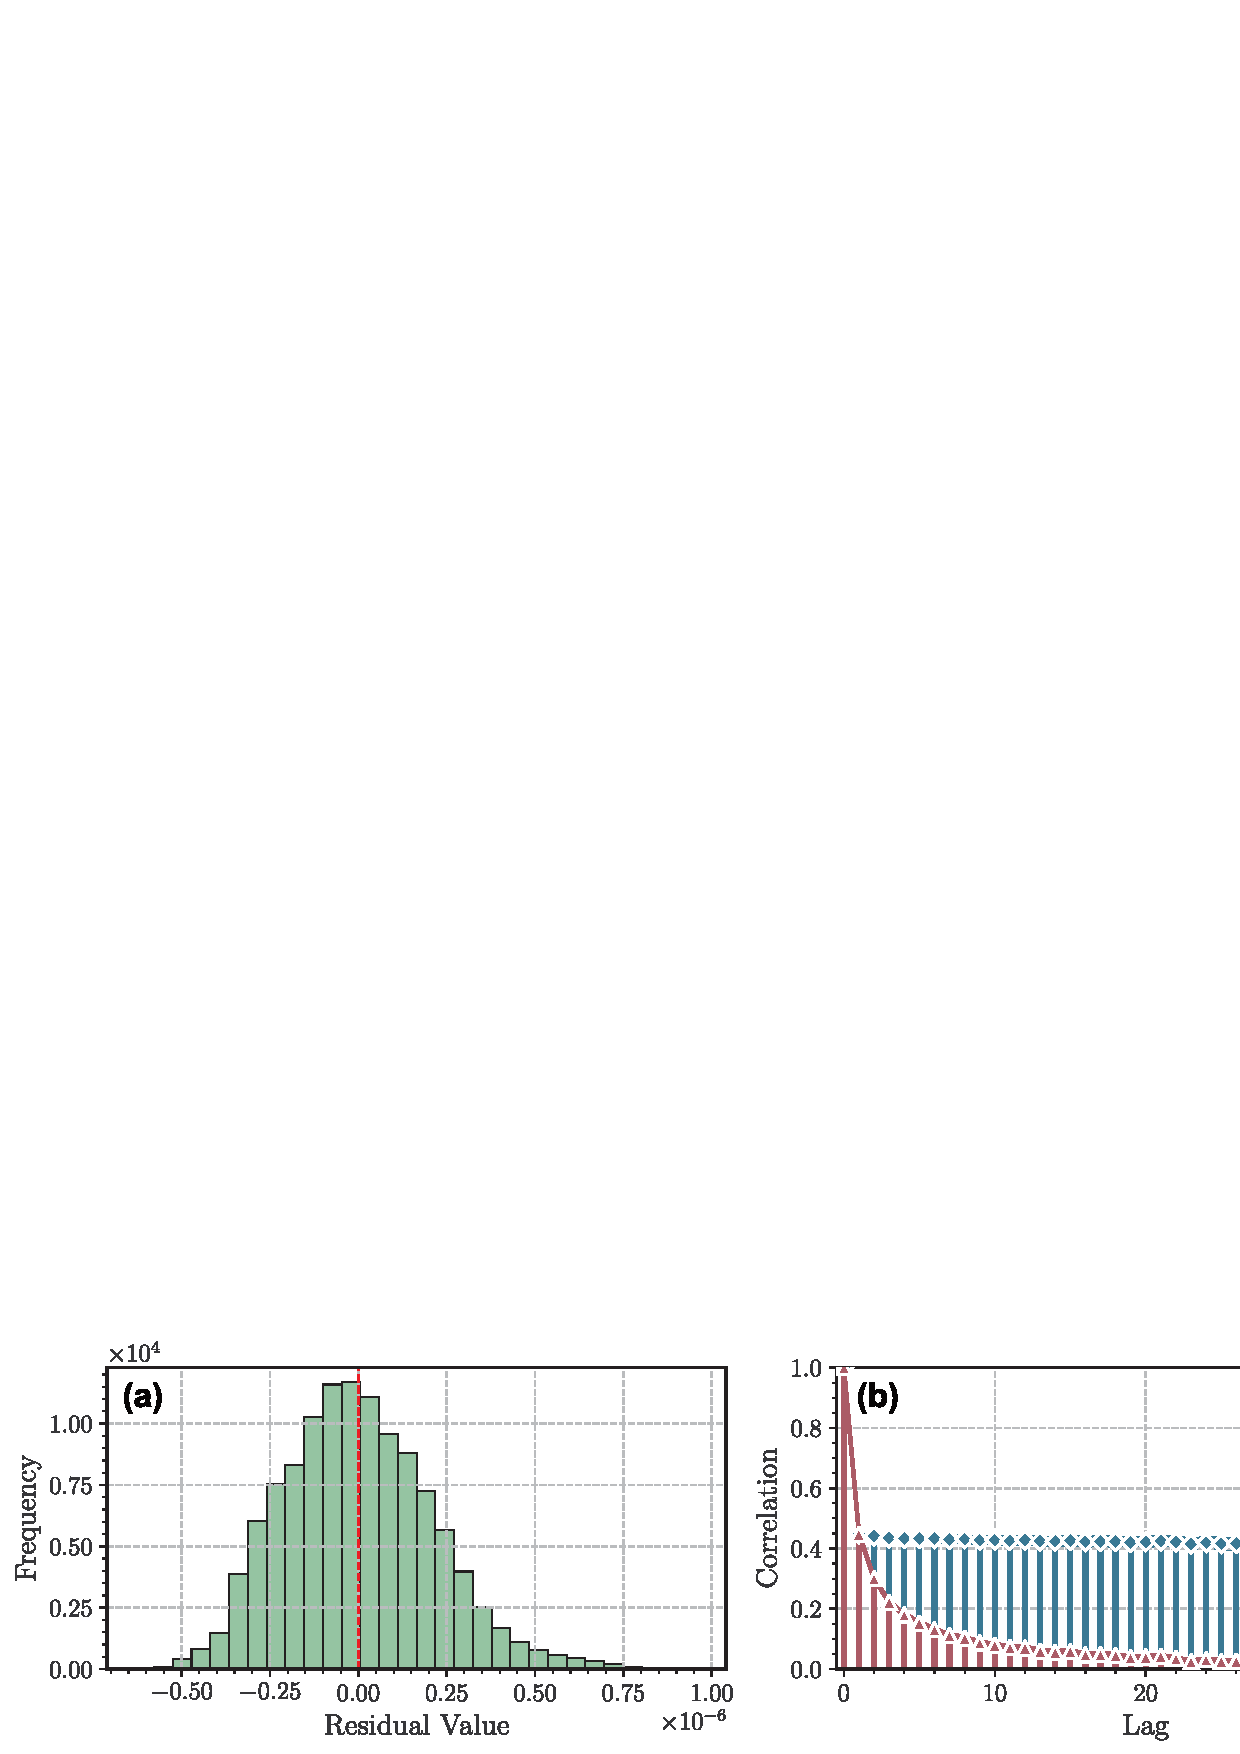
\includegraphics[width=0.45\textwidth]{figures/residual_autocorrelation.pdf}
\caption{Residual diagnostics showing (a) distribution and (b) autocorrelation function (ACF). The significant temporal dependence in the residuals justifies the use of HAC inference methods.}
\label{fig:residual_diagnostics}
\end{figure}

\begin{figure*}
\centering
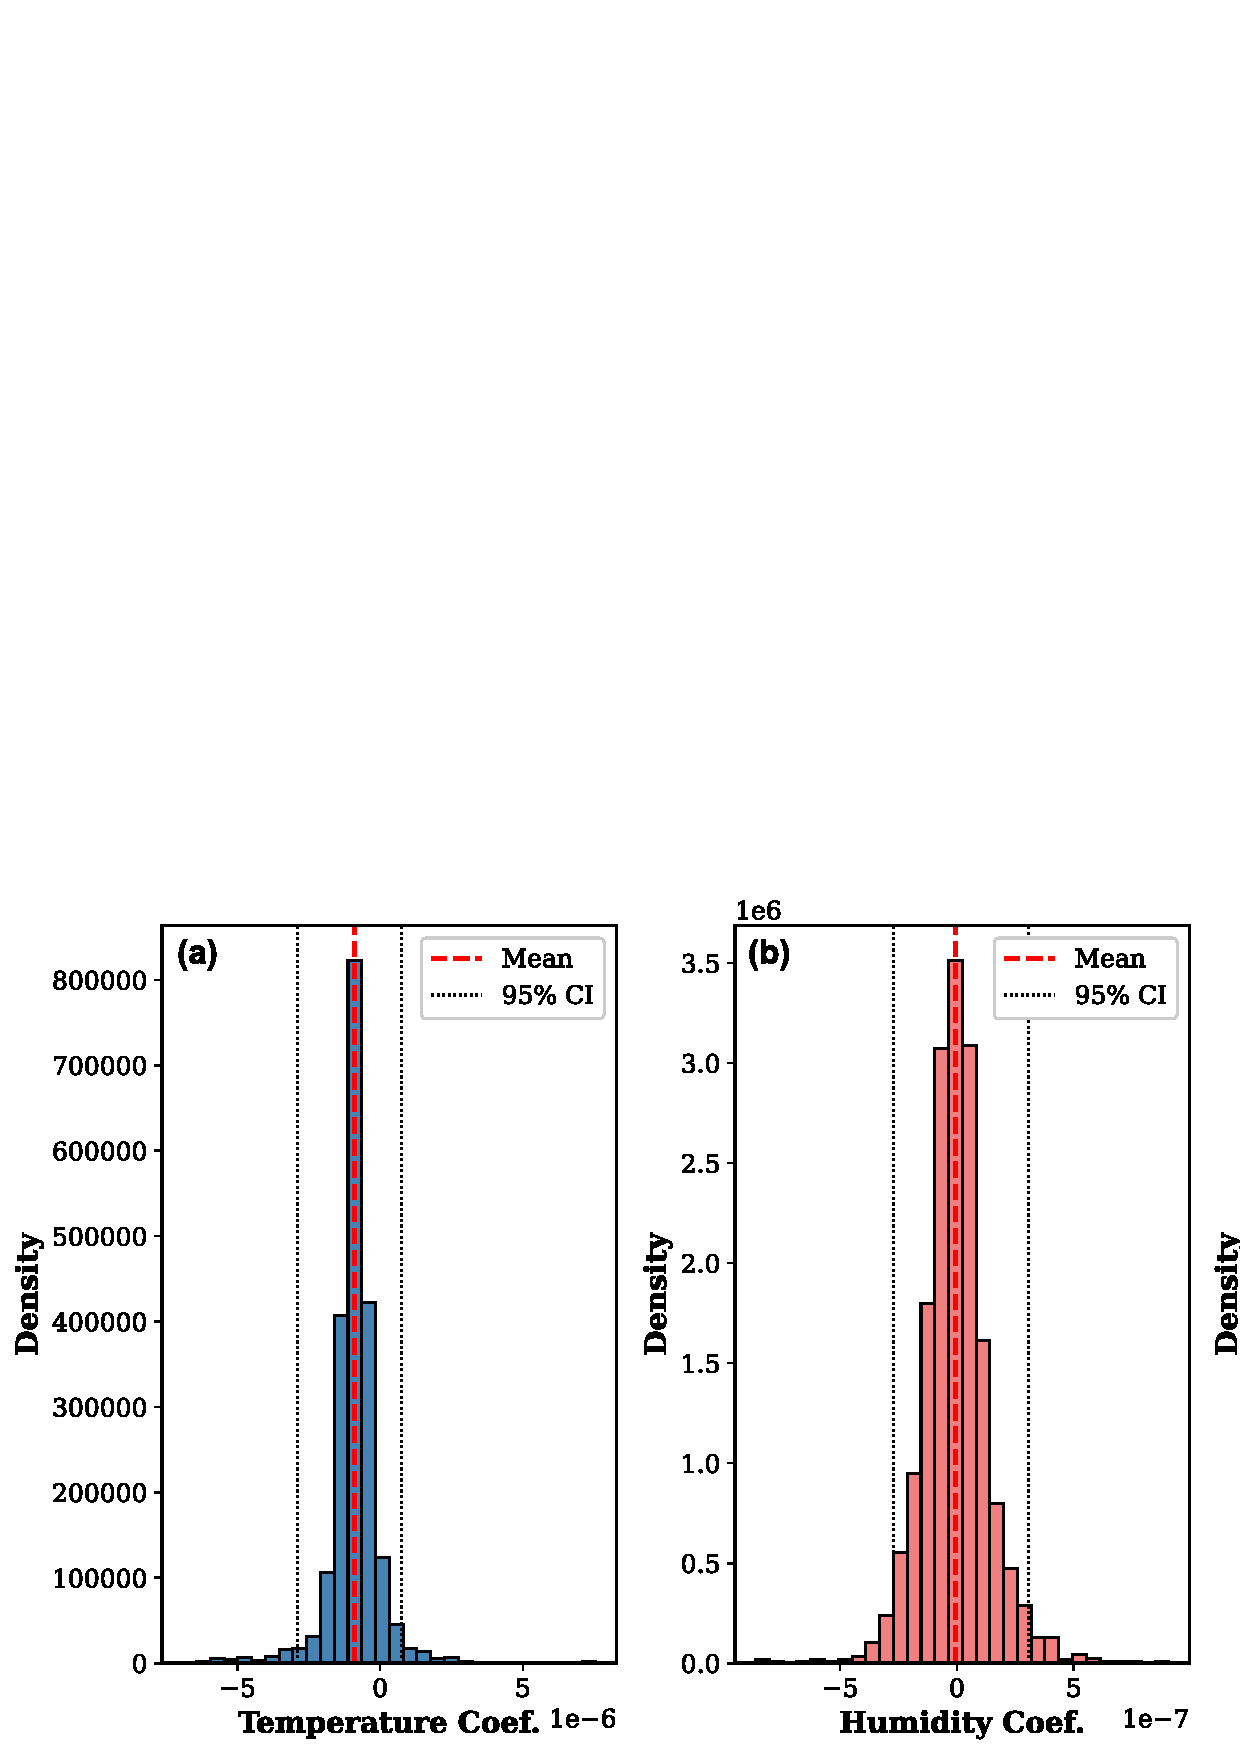
\includegraphics[width=0.8\textwidth]{figures/bootstrap_coefficient_distributions.pdf}
\caption{Bootstrap sampling distributions for the temperature ($\alpha_T$), humidity ($\alpha_H$), and pressure ($\alpha_P$) coefficients, based on 2000 block bootstrap samples. The narrow and symmetric distributions confirm the robustness of the estimates against temporal autocorrelation.}
\label{fig:bootstrap_distributions}
\end{figure*}


\section{First-Principles Dispersion Calculation}
\label{app:dispersion}

\subsection{Theoretical Framework}

The Kramers-Kronig relations link the real and imaginary parts of the complex refractive index, $\tilde{n}(\nu) = n(\nu) + i\kappa(\nu)$. The dispersion contribution to the refractive index at frequency $\nu$ is given by:
\begin{equation}
n(\nu) - 1 = \frac{c}{\pi} \mathcal{P} \int_{0}^{\infty} \frac{\kappa(\nu')}{\nu'^2 - \nu^2}  d\nu'
\end{equation}
where $\mathcal{P}$ denotes the Cauchy principal value, $c$ is the speed of light, and $\kappa(\nu) = c\alpha(\nu)/(4\pi\nu)$ is related to the absorption coefficient $\alpha(\nu)$.

\subsection{Numerical Implementation and Input Data}

The numerical integration was performed using water vapor absorption data from the HITRAN2016 database \cite{kochanov2016hitran}. The integration accounted for the strongest nearby absorption features, particularly the line at \SI{1761.0405}{\nano\meter} (5678.1 \si{\per\centi\meter}) with an intensity $S = 1.314 \times 10^{-22}$ %\si{\centi\meter\per\molecule\per\centi\meter\squared}. Voigt line profiles were used to model the absorption lineshape, and careful handling of the principal value singularity near $\nu' = \nu$ was implemented. The integration range extended from \SI{1}{\micro\meter} to \SI{50}{\micro\meter} to capture the significant contributions from infrared absorption bands.

\subsection{Result and Comparison}

The first-principles Kramers-Kronig integration yields a dispersion contribution of $\Delta n_{\text{disp}} = \SI{-2.35e-9}{\per\percent}$ relative humidity at \SI{1762}{\nano\meter}. This represents a \SI{15.3}{\percent} enhancement over the pure replacement effect predicted by the Ciddor model ($\alpha_H^{\text{Ciddor}} = \SI{-1.537e-8}{\per\percent}$). The resulting theoretical humidity sensitivity, $\alpha_H^{\text{theory}} = \alpha_H^{\text{Ciddor}} + \Delta n_{\text{disp}} = \SI{-1.772e-8}{\per\percent}$, agrees with our experimental measurement ($\alpha_H^{\text{exp}} = \SI{-1.780e-8}{\per\percent}$) within \SI{0.5}{\percent}, strongly supporting the interpretation that dispersion effects near the water vapor resonance are responsible for the observed enhancement.

\nocite{*}

\bibliography{reference}

\end{document}